\begin{practice}
    \subsection{Luyện tập}

    \begin{questions}[resume=SBT]
        \item Những hình nào dưới đây là đa giác đều?
        \begin{tasks}[label=\alph*)](2)
            \task Tam giác đều;
            \task Hình vuông;
            \task Hình tròn;
            \task Hình bình hành;
            \task Hình chữ nhật;
            \task Lục giác đều.
        \end{tasks}

        \answerline

        \item Hình phẳng nào dưới đây có dạng đa giác đều?

        \begin{center}
            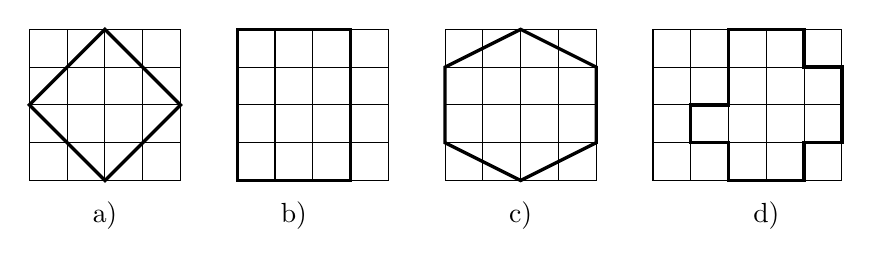
\begin{tikzpicture}[x=0.48cm,y=0.48cm]
                \begin{scope}[shift={(0,0)}]
                    \draw[step=1] (0,0) grid (4,4);
                    \draw[very thick] (2,4)--(4,2)--(2,0)--(0,2)--cycle;
                    \node[below=4pt] at (2,0) {a)};
                \end{scope}
                \begin{scope}[shift={(5.5,0)}]
                    \draw[step=1] (0,0) grid (4,4);
                    \draw[very thick] (0,0) rectangle (3,4);
                    \node[below=4pt] at (1.5,0) {b)};
                \end{scope}
                \begin{scope}[shift={(11,0)}]
                    \draw[step=1] (0,0) grid (4,4);
                    \draw[very thick] (0,3)--(2,4)--(4,3)--(4,1)--(2,0)--(0,1)--cycle;
                    \node[below=4pt] at (2,0) {c)};
                \end{scope}
                \begin{scope}[shift={(16.5,0)}]
                    \draw[step=1] (0,0) grid (5,4);
                    \draw[very thick]
                        (1,1)--(1,2)--(2,2)--(2,4)--(4,4)--(4,3)--
                        (5,3)--(5,1)--(4,1)--(4,0)--(2,0)--(2,1)--cycle;
                    \node[below=4pt] at (3,0) {d)};
                \end{scope}
            \end{tikzpicture}

            \textit{Hình 9.12}
        \end{center}

        \answerline

        \item Hình nào dưới đây vẽ hai điểm $M$, $N$ thoả mãn phép quay ngược chiều $60^\circ$ tâm $O$ biến $N$ thành $M$?

        \begin{center}
            \begin{tikzpicture}[x=1cm,y=1cm]
                \begin{scope}[shift={(0,0)}]
                    \coordinate (Oa) at (0,0);
                    \coordinate (Ma) at (2.2,0);
                    \coordinate (Na) at (60:1.7);
                    \draw (Oa)--(Ma) (Oa)--(Na);
                    \draw (0.45,0) arc[start angle=0,end angle=60,radius=.45];
                    \draw (1.08,-.08)--(1.08,.08);
                    \draw ($(Oa)!0.55!(Na)+(-.10,.04)$)--($(Oa)!0.55!(Na)+(.08,-.05)$);
                    \draw ($(Oa)!0.55!(Na)+(-.06,.12)$)--($(Oa)!0.55!(Na)+(.12,.03)$);
                    \node[below left] at (Oa) {$O$};
                    \node[right] at (Ma) {$M$};
                    \node[above] at (Na) {$N$};
                    \node at (.56,.30) {$60^\circ$};
                    \node[below=7pt] at (1.05,0) {a)};
                \end{scope}
                \begin{scope}[shift={(4.2,0)}]
                    \coordinate (Ob) at (0,0);
                    \coordinate (Mb) at (10:2.1);
                    \coordinate (Nb) at (70:2.1);
                    \draw (Ob)--(Mb) (Ob)--(Nb);
                    \draw (10:.45) arc[start angle=10,end angle=70,radius=.45];
                    \draw ($(Ob)!0.55!(Mb)+(-.02,-.09)$)--($(Ob)!0.55!(Mb)+(.02,.09)$);
                    \draw ($(Ob)!0.55!(Nb)+(-.09,.03)$)--($(Ob)!0.55!(Nb)+(.09,-.03)$);
                    \node[below left] at (Ob) {$O$};
                    \node[right] at (Mb) {$M$};
                    \node[above] at (Nb) {$N$};
                    \node at (.55,.38) {$60^\circ$};
                    \node[below=7pt] at (1.05,0) {b)};
                \end{scope}
                \begin{scope}[shift={(8.6,0)}]
                    \coordinate (Oc) at (0,0);
                    \coordinate (Nc) at (15:2.1);
                    \coordinate (Mc) at (65:2.1);
                    \draw (Oc)--(Nc) (Oc)--(Mc);
                    \draw (15:.45) arc[start angle=15,end angle=65,radius=.45];
                    \draw ($(Oc)!0.55!(Nc)+(-.02,-.09)$)--($(Oc)!0.55!(Nc)+(.02,.09)$);
                    \draw ($(Oc)!0.55!(Mc)+(-.09,.03)$)--($(Oc)!0.55!(Mc)+(.09,-.03)$);
                    \node[below left] at (Oc) {$O$};
                    \node[right] at (Nc) {$N$};
                    \node[above] at (Mc) {$M$};
                    \node at (.55,.34) {$50^\circ$};
                    \node[below=7pt] at (1.05,0) {c)};
                \end{scope}
                \begin{scope}[shift={(13,0)}]
                    \coordinate (Od) at (0,0);
                    \coordinate (Nd) at (2.1,0);
                    \coordinate (Md) at (60:2.1);
                    \draw (Od)--(Nd) (Od)--(Md);
                    \draw (0.45,0) arc[start angle=0,end angle=60,radius=.45];
                    \draw ($(Od)!0.55!(Nd)+(-.02,-.09)$)--($(Od)!0.55!(Nd)+(.02,.09)$);
                    \draw ($(Od)!0.55!(Md)+(-.09,.03)$)--($(Od)!0.55!(Md)+(.09,-.03)$);
                    \node[below left] at (Od) {$O$};
                    \node[right] at (Nd) {$N$};
                    \node[above] at (Md) {$M$};
                    \node at (.55,.30) {$60^\circ$};
                    \node[below=7pt] at (1.05,0) {d)};
                \end{scope}
            \end{tikzpicture}

            \textit{Hình 9.13}
        \end{center}

        \answerline

        \item Cho lục giác đều $ABCDEF$ nội tiếp một đường tròn $(O)$. Chứng minh rằng điểm $O$ cách đều tất cả các cạnh của lục giác đều.

        \answerline
        \answerline
        \answerline

        \item Cho một bát giác đều (đa giác đều có 8 cạnh) nội tiếp một đường tròn tâm $O$. Kẻ các đoạn thẳng nối $O$ với các đỉnh của đa giác và chia đa giác thành 8 tam giác nhỏ cân tại đỉnh $O$. Ba góc của mỗi tam giác nhỏ có số đo bằng bao nhiêu?

        \answerline
        \answerline

        \item Cho $A'$, $B'$, $C'$, $D'$, $E'$, $F'$ là trung điểm các cạnh $AB$, $BC$, $CD$, $DE$, $EF$, $FA$ của lục giác đều $ABCDEF$. Chứng minh rằng $A'B'C'D'E'F'$ là một lục giác đều.

        \answerline
        \answerline
        \answerline

        \item Cho tam giác đều $ABC$ nội tiếp đường tròn $(O)$ như Hình 9.14. Hãy cho biết các phép quay thuận chiều lần lượt $120^\circ$; $240^\circ$; $360^\circ$ với tâm $O$ biến các đỉnh $A$, $B$, $C$ thành những điểm nào.

        \begin{center}
            \begin{tikzpicture}[scale=0.8]
                \coordinate (O) at (0,0);
                \coordinate (A) at (90:2);
                \coordinate (B) at (210:2);
                \coordinate (C) at (330:2);
                \draw (O) circle (2);
                \draw (A)--(B)--(C)--cycle;
                \draw (O)--(A) (O)--(B) (O)--(C);
                \fill (O) circle (1.2pt);
                \node[above=1pt of A] {$A$};
                \node[left=1pt of B] {$B$};
                \node[right=1pt of C] {$C$};
                \node[below right=1pt of O] {$O$};
                \node[left=3pt] at (-.45,.40) {$120^\circ$};
            \end{tikzpicture}

            \textit{Hình 9.14}
        \end{center}

        \answerline
        \answerline

        \item Cho hình vuông $ABCD$ nội tiếp đường tròn $(O)$ như Hình 9.15. Hãy cho biết các phép quay ngược chiều lần lượt $90^\circ$; $180^\circ$; $270^\circ$; $360^\circ$ với tâm $O$ biến các đỉnh $A$, $B$, $C$, $D$ thành những điểm nào.

        \begin{center}
            \begin{tikzpicture}[scale=0.8]
                \coordinate (O) at (0,0);
                \coordinate (A) at (-1.35,1.35);
                \coordinate (B) at (1.35,1.35);
                \coordinate (C) at (1.35,-1.35);
                \coordinate (D) at (-1.35,-1.35);
                \draw (O) circle ({1.35*sqrt(2)});
                \draw (A)--(B)--(C)--(D)--cycle;
                \draw (A) ++(.18,0)--++(0,-.18)--++(-.18,0);
                \draw (B) ++(-.18,0)--++(0,-.18)--++(.18,0);
                \draw (C) ++(-.18,0)--++(0,.18)--++(.18,0);
                \draw (D) ++(.18,0)--++(0,.18)--++(-.18,0);
                \fill (O) circle (1.2pt);
                \node[below left=2pt of O] {$O$};
                \node[above left=1pt of A] {$A$};
                \node[above right=1pt of B] {$B$};
                \node[below right=1pt of C] {$C$};
                \node[below left=1pt of D] {$D$};
            \end{tikzpicture}

            \textit{Hình 9.15}
        \end{center}

        \answerline
        \answerline

        \item Cho lục giác đều $ABCDEF$ nội tiếp đường tròn tâm $O$.
        \begin{questions}
            \item Chứng tỏ $ACE$ là tam giác đều.

            \answerline
            \answerline
            \item Liệt kê ba phép quay giữ nguyên tam giác đều $ACE$.

            \answerline
            \item Liệt kê sáu phép quay giữ nguyên lục giác đều $ABCDEF$.

            \answerline
        \end{questions}

        \item Một phép quay thuận chiều $120^\circ$ tâm $O$ biến điểm $A$ thành điểm $B$, biến điểm $B$ thành điểm $C$. Chứng tỏ rằng $ABC$ là tam giác đều nội tiếp một đường tròn tâm $O$.

        \answerline
        \answerline
        \answerline

        \item Cho $O$ là trung điểm của đoạn thẳng $AB$.
        \begin{questions}
            \item Tìm một phép quay biến điểm $A$ thành điểm $B$ và biến điểm $B$ thành điểm $A$.

            \answerline
            \item Phép quay thuận chiều $90^\circ$ tâm $O$ biến $A$ thành $C$ và biến $B$ thành $D$. Chứng tỏ rằng $ACBD$ là một hình vuông.

            \answerline
            \answerline
            \answerline
        \end{questions}
    \end{questions}
\end{practice}
